\chapter{Data Sample, Event Selection, and Jet Definitions}\label{ch:data_and_event_selection}

\section{Data sample}\label{sec:data}
This analysis uses the entirety of the 2015 and 2016 ATLAS datasets, comprising \linebreak $36.1~fb^{-1}~(\pm2.1\%)$ of integrated luminosity, with $\sqrt{s}=13~TeV$.
A \textit{good runs list} (GRL) is used to select only those data-taking periods in which alld detectors are fully functional~\cite{data-grl}.

\section{Trigger}\label{sec:trigger}
Events are required to pass an $H_{T}$-based trigger, where $H_{T}$ is the scalar sum of the $p_{T}$ of all jets in an event.
The jets used for the calculation of $H_{T}$ in the trigger are level-one jets with $p_{T}>100~GeV$.
To pass the trigger, an event must have $H_{T}>1~TeV$.
Figure~\ref{fig:trigger_efficiency} shows the trigger efficiency versus large-$R$ jet $p_{T}$ threshold for events with $\geq4$ and $\geq5$ large-$R$ jets.
For events with five or more large-$R$ jets, the trigger efficiency is $100\%$ when the jet $p_{T}$ threshold is $200~GeV$ or above.
For events with four or more jets, an additional requirement on the leading jet $p_{T}$ is needed to ensure full trigger efficiency at this jet-$p_{T}$ threshold.
For the $\geq4$-jet regions, the leading jet will be required to have a $p_{T}$ of at least $440~GeV$.

\begin{figure}[!ht]
    \centering
    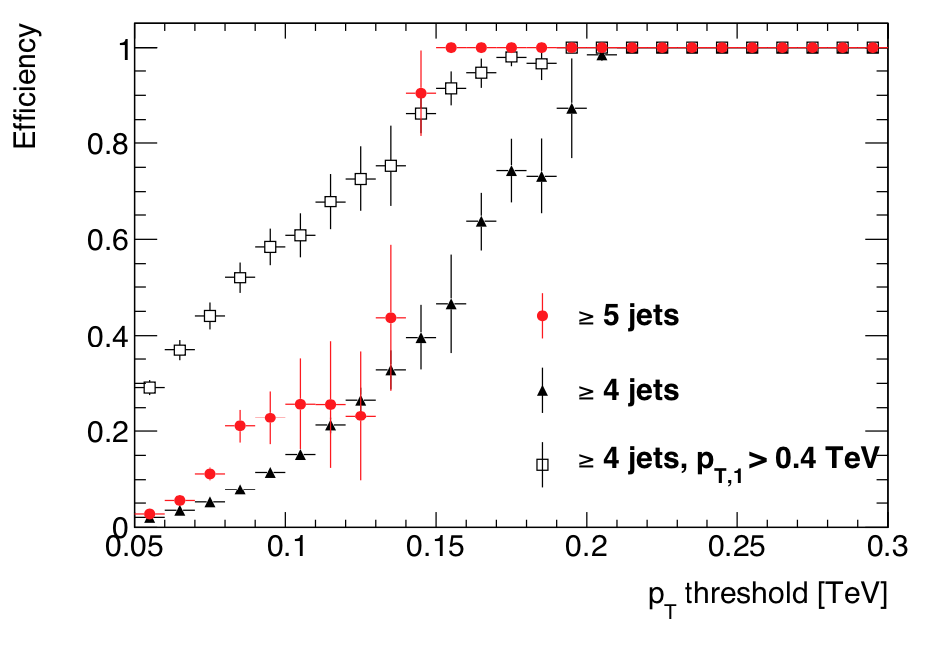
\includegraphics[width=0.9\textwidth]{data_trigger_efficiency}
    \caption{Trigger efficiency versus large-$R$ jet $p_{T}$ threshold for events with $\geq4$ and $\geq5$ large-$R$ jets.
    For events with $\geq4$ large-$R$ jets, and additional requirement of leading-jet $p_{T}>400~GeV$ ensures $100\%$ trigger efficiency.
    }
    \label{fig:trigger_efficiency}
\end{figure}

\section{Event selection}\label{sec:event_selection}

Events considered by this analysis must meet the following pre-selection criteria:

\begin{itemize}
    \item In the list of good luminosity blocks in the GRL as described in~\ref{sec:data}.
    \item No errors in the LAr or tile calorimeters or the inner detector when the events were measured
    \item Pass the $H_{T}$ trigger as described in~\ref{sec:trigger}.
    \item At least one primary vertex from at least two tracks with $p_{T}>400~MeV$ each
    \item At least one large-$R$ jet (see~\ref{sec:jet_definitions}) with $p_{T}>440~GeV$
\end{itemize}

\section{Jet definitions, $b$-tagging, and $b$-matching}\label{sec:jet_definitions}

In this analysis, two different types of jets are defined.
Large-$R$ jets are reconstructed using the anti-$k_{T}$ algorithm with $R=1.0$ and are trimmed by re-clustering the constituents of each jet with $R_{sub-jet}=0.2$ and rejecting any sub-jet with $p_{T}^{sub-jet}/p_{T}^{jet}<0.05$.
The trimmed large-$R$ jets are required to have $p_{T}>200~GeV$.

Small-$R$ jets are reconstructed using the anti-$k_{T}$ algorithm with $R=0.4$.
To be considered for b-tagging, a small-R jet must have $p_{T}$ of at least $50~GeV$ and $|\eta|$ less than $2.5$.
The fixed-efficiency $70\%$ working point is used for $b$-tagging.

Only large-$R$ jets are used for the analysis, but the $b$-tagging algorithm is only calibrated for small-$R$ jets.
So a matching procedure is used to identify large-$R$ jets that can be associated with a $b$-tagged small-$R$ jet.
Large-$R$ jets found to be within $\Delta R=1.0$ of a $b$-tagged small-$R$ jet in the same event are referred to as $b$-matched jets.
Jet mass templates are derived separately for $b$-matched and non-$b$-matched jets.

For details of how jets are reconstructed, trimmed, and calibrated, as well as the definition of different jet parameters, see chapter~\ref{ch:jets}.
The algorithm used to identify $b$-jets is described in chapter~\ref{subsec:jet_b_tagging} as well as~\cite{b-jet-perf-1,b-jet-perf-2}.

The control, validation, and signal regions defined in section~\ref{sec:region_defs} can be segmented into $b$-tag and $b$-veto regions.
Events with at least one $b$-tagged small-$R$ jet are considered $b$-tag events, while those without are labelled as $b$-veto.
When $b$-tagging is not part of the selection requirements for a region, it is called a $b$-inclusive region.

\section{Control, signal, validation, and uncertainty determination regions} \label{sec:region_defs}
Events are divided into control, signal, validation, and uncertainty determination regions.
Figure~\ref{fig:workflow} illustrates how the different regions are used in the analysis.
Jet mass templates are constructed from control region (CR) events and used predict the mass distribution in the uncertainty determination region (UDR), validation region (VR), and signal region (SR), as discussed in section~\ref{sec:jet_mass_templates}.
The discrepancy between predicted and observed jet masses in the UDR is taken as the systematic uncertainty of the background estimation method.
Observed and predicted masses in the validation regions can be compared to check that any discrepancy falls within this uncertainty, as a way of validating the method.
Finally the observed yields in the signal region can be compared to the predicted background yield in the signal region.

\begin{figure}[!ht]
    \centering
    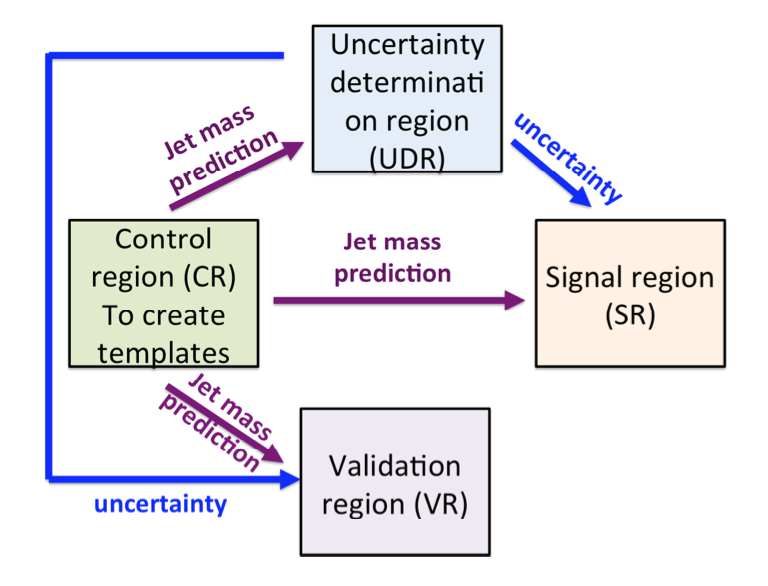
\includegraphics[width=0.9\textwidth]{background_workflow}
    \caption{Workflow illustrating how the different regions are used in the analysis.}
    \label{fig:workflow}
\end{figure}

Table~\ref{tbl:region_defs} gives the cuts used to define each of these regions.
Control region events are required to have exactly three large-$R$ jets each with $p_{T}>200~GeV$.
If a control region event has at least one $b$-matched large-$R$ jet, the additional requirement of $|\Delta\eta_{12}|>1.4$ is applied, in order to suppress potential signal contamination.

There are a total of five partially-overlapping signal regions, all of which require $|\Delta\eta_{12}|<1.4$.
Regions are defined by the minimum number of large-$R$ jets required ($N_{jet}$), by whether or not a $b$-tagged jet is required to be present in the event, and by a minimum requirement on $M_{J}^{\Sigma}$.
There are two signal regions which require four or more large-$R$ jets with $p_{T}>200~GeV$, and three signal regions which require five or more.
Four-jet signal regions require the $p_T$ of the leading large-$R$ jet to be greater than $400~GeV$.
The $b$-tag signal regions each require at least one $b$-tagged small-$R$ jet per event, and are the most sensitive to the RPV gluino direct and cascade decay models.
Signal regions without the $b$-tag requirement are also defined, referred to as inclusive signal regions.
These inclusive regions are less sensitive to the RPV gluino decay signal, but can be sensitive to other potential BSM signals.

The minimum value of $M_{J}^{\Sigma}$ for each signal region is optimized based on signal sensitivity separately for each signal region.
For the 5-jet $b$-tag signal region, the optimal $M_{J}^{\Sigma}$ cut is $0.8~TeV$ for the cascade decay model, and $0.6~TeV$ for the direct decay model.
The signal regions corresponding to these two $M_{J}^{\Sigma}$ cuts will be referred to as 5jSRb1 and 5jSRb2, respectively.

The difference between the signal and validation regions is a reversal of the $|\Delta\eta_{12}|$ requirement, and removal of the $M_{J}^{\Sigma}$ requirement.
Requiring large $|\Delta\eta|_{12}$ reduces the signal contribution to these high-multiplicity regions.
There is no $M_{J}^{\Sigma}$ requirement for the validation region, so that the performance of the template method over the full range of $M_{J}^{\Sigma}$ can be evaluated.

There are two uncertainty determination regions (UDRs), which are used to derive the data-driven background systematic uncertainty.
The high-$p_{T}$ UDR, referred to as as UDR1, consists of events with exactly two large-R jets, with at least one having $p_{T}>400~GeV$.
The low-$p_{T}$ UDR, referred to as UDR2, consists of events with exactly four large-R jets, all of which have $p_{T}<400~GeV$.
The UDRs are independent of the control, validation, and signal regions.

\begin{table}
    \centering

    \begin{tabular}{cccccccc}

        \toprule
                             &                        & $N_{jet}~(p_T>200~GeV)$ & $b$-tag & $b$-match & $p_{T,1}$  & $|\Delta\eta_{12}|$ & $M_{J}^{\Sigma}$ \\
        \midrule
        \multirow{2}{*}{CR}  & 3jCRb                  & $=3$                    & -       & Yes       & -          & -                   & - \\
                             & 3jCR                   & $=3$                    & -       & No        & -          & -                   & - \\
        \midrule
        \multirow{2}{*}{UDR} & UDR1                   & $=2$                    & -       & -         & $>400~GeV$ & -                   & - \\
                             & UDR2                   & $=4$                    & -       & -         & $<400~GeV$ & -                   & - \\
        \midrule
        \multirow{4}{*}{VR}  & 4jVRb                  & $\geq4$                 & Yes     & -         & $>400~GeV$ & $>1.4$              & - \\
                             & 5jVRb                  & $\geq5$                 & Yes     & -         & -          & $>1.4$              & - \\
                             & 4jVR                   & $\geq4$                 & -       & -         & $>400~GeV$ & $>1.4$              & - \\
                             & 5jVR                   & $\geq5$                 & -       & -         & -          & $>1.4$              & - \\
        \hline
        \multirow{5}{*}{SR}  & 4jSRb                  & $\geq4$                 & Yes     & -         & $>400~GeV$ & $<1.4$              & $>1.0~TeV$ \\
                             & \multirow{2}{*}{5jSRb} & $\geq5$                 & Yes     & -         & -          & $<1.4$              & $>0.8~TeV$ \\
                             &                        & $\geq5$                 & Yes     & -         & -          & $<1.4$              & $>0.6~TeV$ \\
                             & 4jSR                   & $\geq4$                 & -       & -         & $>400~GeV$ & $<1.4$              & $>1.0~TeV$ \\
                             & 5jSR                   & $\geq5$                 & -       & -         & -          & $<1.4$              & $>0.8~TeV$ \\
        \bottomrule
    \end{tabular}

    \caption{Summary of the requirements defining the control, uncertainty determination, validation, and signal regions.
    Requirements are placed on the large-R jet multiplicity ($N_{jet}$), the presence or absence of a b-tagged small-R jet ($b$-tag),
    the $p_T$ of the leading jet ($p_{T,1}$), the pseudorapidity difference between the two leading jets ($|\Delta\eta_{12}|$),
    and the scalar sum of the first four leading jets in the event ($M_J^{\Sigma}$)~\cite{paper-plb}.}
    \label{tbl:region_defs}

\end{table}
